\documentclass{article}
\usepackage{amsmath,amsthm,amssymb,graphicx,pgf,verbatim,minted,comment,hyperref}
\usemintedstyle{friendly}

\newcommand{\N}{\mathbb{N}}
\newcommand{\R}{\mathbb{R}}
\newcommand{\ZZ}{\mathbb{Z}}
\newcommand{\Q}{\mathbb{Q}}
\newcommand{\C}{\mathbb{C}}
\newcommand{\F}{\mathbb{F}}
\newcommand{\alp}{\alpha}
\newcommand{\bb}{\beta}
\newcommand{\zz}{\zeta}
\newcommand{\OO}{\mathscr{O}}
\newcommand{\PP}{\mathscr{P}}
\newcommand{\QQ}{\mathscr{Q}}
\newcommand{\diff}{\mathrm{d}}
\newcommand{\tr}{\mathrm{Tr}}
\renewcommand{\d}{\displaystyle} 
\DeclareMathOperator{\A}{A}
\DeclareMathOperator{\mat}{Mat}
\newtheorem{thm}{Theorem}[section]
\newtheorem{defi}{Definition}[section]
\newtheorem{prop}{Proposition}[section]
\newtheorem{lem}{Lemma}[section]
\newtheorem{cor}{Corollary}[section]
\newtheorem{rmk}{Remark}[section]
\def\floor(#1){\lfloor #1 \rfloor}                                                          % floor function
\def\bfloor(#1){\bigg\lfloor #1 \bigg\rfloor}
\def\bg(#1){\big( #1 \big) }                                           		 % big '(' and ')'
\def\bgg(#1){\bigg( #1 \bigg) }                                                           % bigg '(' and ')'
\def\rbg(#1){\big[ #1 \big] }                                           		 % big '[' and ']'
\def\rbgg(#1){\bigg[ #1 \bigg] }                                                          % bigg '[' and ']'

\begin{document} 

\title{\bf ML Homework 5}
\author{\bf Bo-Cheng Huang, 309652022}
\date{}

\maketitle


\section{Gaussian Process}

\subsection{Code with detailed explanations}

$\quad\ $For Part 1, I use a rational quadratic kernel to compute similarities between different points. It is parameterized by a length scale parameter $l > 0$ and a scale mixture parameter $\alpha > 0$. The formula of a rational quadratic kernel is 
\[
k(x_i,x_j)={\bigg(1+\frac{d(x_i,x_j)^2}{2 \alpha l^2}\bigg)}^{-\alpha}
\]
where $d$ is the Euclidean distance.

\begin{listing}[!ht]
\begin{minted}[linenos,mathescape]{python}
def kernel(X1,X2,l,alpha):
    '''
    Impletation of rational quadratic kernel
    X1: (n)-array
    X2: (m)-array
    return a (n,m)-array
    ''' 
    sqeddist=np.power(X1.reshape(-1,1)-X2.reshape(1,-1),2)
    return np.power((1+sqeddist/(2*alpha*l**2)),-alpha)
\end{minted}
\caption{Kernel}
\label{listing}
\end{listing}

Hence I can predict the distribution of $f$ by rational quadratic kernel. For $\mathbf{f}={[f(x_1),\dots,f(x_N)]}^T$ and $\mathbf{y}={[y_1,\dots,y_N],}^T$ let
\[
p(\mathbf{y}|\mathbf{f})=\mathcal{N}(\mathbf{y}|\mathbf{f},\beta^{-1}\mathbf{I}_N),\ p(\mathbf{f})=\mathcal{N}(\mathbf{0}, \mathbf{K}),\ p(\mathbf{y})=\mathcal{N}(\mathbf{y}|\mathbf{0}, \mathbf{C}),
\]
where $\mathbf{C}(\mathbf{x}_n,\mathbf{x}_m)=k(\mathbf{x}_n,\mathbf{x}_m)+\beta^{-1}\delta_{nm}$. Then the conditional distribution $p(y^*|\mathbf{y})$ is a Gaussian distibution with:
\begin{align*}
\mu(\mathbf{x}^*)&={k(\mathbf{x},\mathbf{x}^*)}^T\mathbf{C}^{-1}\mathbf{y},\\
\sigma^2(\mathbf{x}^*)&=k^*-{k(\mathbf{x},\mathbf{x}^*)}^T\mathbf{C}^{-1}k(\mathbf{x},\mathbf{x}^*),\\
k^*&=k(\mathbf{x}^*,\mathbf{x}^*)+\beta^{-1}.
\end{align*}

So I can do the Gaussian process of predicting the distribution of $f$ in Listing 2 and Listing 3 is the code for data preprocessing and visualization:

\begin{listing}[!ht]
\begin{minted}[linenos,mathescape]{python}
def predict_GP(X_old,X_new,y,C,beta,l,alpha):
    '''
    Use train data (old) and test data (new) to compute new mean 
    and variance.
    X_old: (n)-array, train data
    X_new: (m)-array, test data
    y: (n)-array, ground truth
    K: (n,n)-array, covariance matrix C
    beta, l, alpha: parameters
    return (len(X_new),1)-array, (len(X_new),1)-array
    '''
    ker_on=kernel(X_old,X_new,l,alpha)
    ker_nn=kernel(X_new,X_new,l,alpha)
    mean=ker_on.transpose()@inv(C)@y.reshape(-1,1)
    ker_star=ker_nn+1/beta*np.identity(len(ker_nn))
    var=ker_star-ker_on.transpose()@inv(C)@ker_on
    return mean,var
\end{minted}
\caption{Gaussian Process}
\label{listing}
\end{listing}

\begin{listing}[!ht]
\begin{minted}[linenos,mathescape]{python}
X=np.zeros((34,1))
Y=np.zeros((34,1))
m=0
input_file=open('input.data','rb')
line=input_file.readline()
while line:
    s=line.decode("utf-8")
    x,y=s.split(' ')
    X[m][0]=float(x)
    Y[m][0]=float(y)
    line=input_file.readline()
    m+=1
    
def print_graph():
    plt.plot(xlin,mean,'black')
    plt.xlim(-60,60)
    plt.fill_between(xlin,mean+2*vars,mean-2*vars,color='aquamarine')
    plt.scatter(X,Y)
    plt.show()
\end{minted}
\caption{Data preprocessing and visualization}
\label{listing}
\end{listing}

\newpage

To get the visualization, let xlin be a sample set which contains data points in the range $[-60,60]$, then I can do prediction between origin data and sample to get the graph.
\begin{listing}[!ht]
\begin{minted}[linenos,mathescape]{python}
beta=5
C=kernel(X,X,1,1)+1/beta*np.identity(len(X))
xlin=np.linspace(-60,60,200).transpose()
mean,vars=predict_GP(X,xlin,Y,C,beta,1,1)
mean=mean.reshape(-1)
vars=np.sqrt(np.diag(vars))
print_graph()
\end{minted}
\caption{Main function of Part 1}
\label{listing}
\end{listing}

For Part 2, I need to optimize the kernel parameters by minimizing negative marginal log-likelihood (for rational quadratic kernel, $\theta=[l,\alpha]$),
\begin{align*}
p(\mathbf{y}| \theta)&=\mathcal{N}(\mathbf{y}|\mathbf{0}, \mathbf{C}_\theta),\\
-\mbox{ln }p(\mathbf{y}| \theta)&= \frac{1}{2}\mbox{ln}| \mathbf{C}_\theta | + \frac{1}{2}\mathbf{y}^T {\mathbf{C}_\theta}^{-1}\mathbf{y} + \frac{N}{2} \mbox{ln} (2\pi).
\end{align*}
Using cholesky from numpy.linalg to get the cholesky decomposition of $C$. Then use $L$ to compute the determinant of $C$. $\mbox{inv}(C)$ is the inverse matrix of $C$.
\begin{listing}[!ht]
\begin{minted}[linenos,mathescape]{python}
def nll_fn(X_train,Y_train,beta):
    '''
    X_train: (n)-array
    Y_train: (n)-array
    beta: parameter
    return the value of negative log-likelihood in GP
    '''
    Y_train = Y_train.ravel()
    def obj(theta):  
        C=kernel(X_train,X_train,theta[0],theta[1])\
        +1/beta*np.identity(len(X_train))
        L=cholesky(C)
        value=0.5*np.sum(np.log(np.diagonal(L)))\
        +0.5*Y_train.transpose()@inv(C)@Y_train\
        +0.5*len(X_train)*np.log(2*np.pi)
        return value
    return obj
\end{minted}
\caption{Negative marginal log-likelihood}
\label{listing}
\end{listing}

Next, I use minimize from scipy.optimize to get the parameters $l,\alpha$. Using different initial value of $l$ and $\alpha$ in $[0.01,0.1,1,10,100]$ to avoid some bigger local minimum. And set l\_opt and alpha\_opt to predict $y$.
\begin{listing}[!ht]
\begin{minted}[linenos,mathescape]{python}
value=1e9
for i in range(-2,3):
    for j in range(-2,3):
        res=minimize(nll_fn(X,Y,beta),[10**i, 10**j],\
                bounds=((1e-5, 1e5),(1e-5, 1e5)))
        if res.fun<value:
            value=res.fun
            l_opt,alpha_opt=res.x
            
beta=5
C=kernel(X,X,l_opt,alpha_opt)+1/beta*np.identity(len(X))
xlin=np.linspace(-60,60,200).transpose()
mean,vars=predict_GP(X,xlin,Y,C,beta,l_opt,alpha_opt)
mean=mean.reshape(-1)
vars=np.sqrt(np.diag(vars))
print_graph()
\end{minted}
\caption{Main function of Part 2}
\label{listing}
\end{listing}

\subsection{Experiments settings and results}
$\quad\ $In Part 1, I set xlin equal to np.linspace(-60,60,100), np.linspace(-60,60,200) and np.linspace(-60,60,500). And the visualization of them are below:
\begin{figure}[h!]
\begin{center}
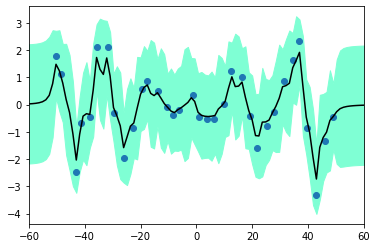
\includegraphics[scale=0.5]{1001.png}
\caption{xlin=np.linspace(-60,60,100)}
\end{center}
\end{figure}
\begin{figure}[h!]
\begin{center}
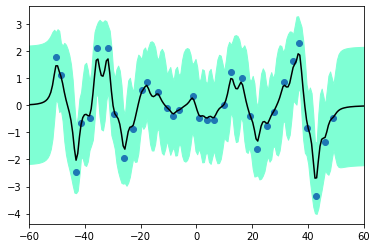
\includegraphics[scale=0.5]{2001.png}
\caption{xlin=np.linspace(-60,60,200)}
\end{center}
\end{figure}
\begin{figure}[h!]
\begin{center}
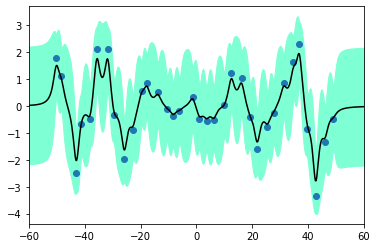
\includegraphics[scale=0.5]{5001.png}
\caption{xlin=np.linspace(-60,60,500)}
\end{center}
\end{figure}

\newpage

In Part 2, I found that l\_opt=2.4468811091753806 and alpha\_opt=901.503494930027. And the visualization of them are below:
\begin{figure}[h!]
\begin{center}
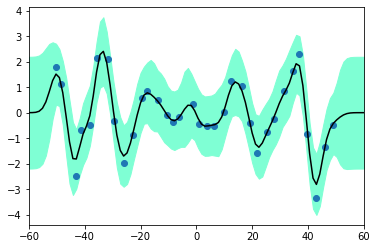
\includegraphics[scale=0.5]{1002.png}
\caption{xlin=np.linspace(-60,60,100)}
\end{center}
\end{figure}
\begin{figure}[h!]
\begin{center}
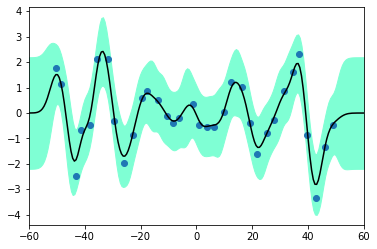
\includegraphics[scale=0.5]{2002.png}
\caption{xlin=np.linspace(-60,60,200)}
\end{center}
\end{figure}
\begin{figure}[h!]
\begin{center}
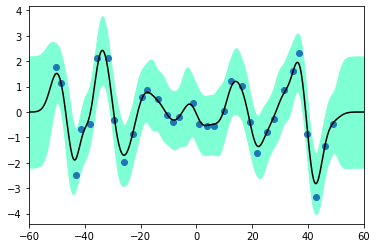
\includegraphics[scale=0.5]{5002.png}
\caption{xlin=np.linspace(-60,60,500)}
\end{center}
\end{figure}

\subsection{Observations and discussion}

$\quad\ $From the visualization of different xlin, when the parameters $l=\alpha=1$, I think that more sample points would make the distribution more smoothing. After using l\_opt and alpha\_opt, the variance of some sample points is smaller than the case $l=\alpha=1$.

\newpage

\section{SVM}

\subsection{Code with detailed explanations}

$\quad\ $First we need to transform data into array.
\begin{listing}[!ht]
\begin{minted}[linenos,mathescape]{python}
def handle_with_csv(x,y,str):
    data=np.zeros((x,y))
    with open(str,newline='') as csvfile:
        rows = csv.reader(csvfile)
        m=0
        for row in rows:
            for i in range(y):
                data[m][i]=float(row[i])
            m+=1
    return data
    
train_x=handle_with_csv(5000,784,'X_train.csv')
train_y=handle_with_csv(5000,1,'Y_train.csv')
test_x=handle_with_csv(2500,784,'X_test.csv')
test_y=handle_with_csv(2500,1,'Y_test.csv')
\end{minted}
\caption{Data preprocessing}
\label{listing}
\end{listing}

In LIBSVM library, I use svm\_train and svm\_predict to do Support Vector Machine. The default type of SVM in LIBSVM is C-SVC and there are 4 types of kernel for users: linear, polynomial, radial basis function and sigmoid.
\begin{itemize}
\item linear: $K(x_i,x_j)=x_i^Tx_j$.
\item polynomial: $K(x_i,x_j)={(\gamma x_i^Tx_j +r)}^d,\ \gamma > 0$.
\item radial basis function: $K(x_i,x_j)=\mbox{exp}(-\gamma {||x_i-x_j||}^2),\ \gamma > 0$.
\item sigmoid: $K(x_i,x_j)=\mbox{tanh}(\gamma x_i^Tx_j +r)$.
\end{itemize}

For Part 1, I use svm\_train with options -t to test different kernels and use svm\_predict to get the accuracy of each model.
\begin{listing}[!ht]
\begin{minted}[linenos,mathescape]{python}
K_type={'linear':'-t 0','polynomial':'-t 1','RBF':'-t 2'}
for parameters in K_type:
    model=svm_train(train_y.reshape(-1),train_x,K_type[parameters])
    p_label,p_acc,p_val=svm_predict(test_y.reshape(-1),test_x,model)
    print('%.2f'%(p_acc[0]),end=' ')
\end{minted}
\caption{Main function of Part 1}
\label{listing}
\end{listing}

For Part 2, to do grid search for finding parameters of the best performing model, I decide some ranges of the parameters of each kernel function. C-SVC is soft-margin SVM, it contains a parameter $C$. In polynomial and RBF kernel, there is a parameter $\gamma$. (I think that the parameters $r=0,\ d=3$ in polynomial kernel have less effect to SVM.)

\begin{listing}[!ht]
\begin{minted}[linenos,mathescape]{python}
for parameters in K_type:
    print(parameters)
    if parameters=='linear':
        for c in range(-9,1):
            model=svm_train(train_y.reshape(-1),train_x,\
                    '-c '+str(2**c)+' '+K_type[parameters])
            p_label,p_acc,p_val=svm_predict(test_y.reshape(-1),test_x,model)
            print('%.2f'%(p_acc[0]),end=' ')
    elif parameters=='polynomial':
        for c in range(-5,5):
            for gamma in range(-9,-3):
                model=svm_train(train_y.reshape(-1),train_x,\
                '-c '+str(2**c)+' -g '+str(2**gamma)+' '+K_type[parameters])
                p_label,p_acc,p_val=svm_predict(test_y.reshape(-1),test_x,model)
                print('%.2f'%(p_acc[0]),end=' ')
            print()
    elif parameters=='RBF':
        for c in range(-3,6):
            for gamma in range(-11,-3):
                model=svm_train(train_y.reshape(-1),train_x,\
                '-c '+str(2**c)+' -g '+str(2**gamma)+' '+K_type[parameters])
                p_label,p_acc,p_val=svm_predict(test_y.reshape(-1),test_x,model)
                print('%.2f'%(p_acc[0]),end=' ')
            print()
    print()
\end{minted}
\caption{Main function of Part 2}
\label{listing}
\end{listing}

In Part 3, I construct a user-defined kernel by linear kernel + RBF kernel. After adding two kernels, it remains to add a column of indexes from 1 to len(X) in front of kernel (the first column).
\begin{listing}[!ht]
\begin{minted}[linenos,mathescape]{python}
def computed_ker(X,gamma):
    '''
    X: (n,m)-array
    gamma: parameter
    return (n,n)-array defined by linear+RBF
    '''
    linear=X@X.transpose()
    RBF=dis.squareform(np.exp(-gamma*dis.pdist(X,'sqeuclidean')))
    ker=linear+RBF
    ker=np.hstack((np.arange(1,len(X)+1).reshape(-1,1),ker))
    return ker
\end{minted}
\caption{User-defined kernel}
\label{listing}
\end{listing}

\newpage

I select $\gamma=2^{-4}$ with good performance in RBF kernel. Then use svm\_problem to transform train\_ker into a legal type to run svm\_train.
\begin{listing}[!ht]
\begin{minted}[linenos,mathescape]{python}
train_ker=computed_ker(train_x,2**-4)
add=svm_problem(train_y.reshape(-1),train_ker,isKernel=True)
p=svm_parameter('-t 4')
model=svm_train(add,p)
test_ker=computed_ker(test_x,2**-4)
p_label,p_acc,p_val=svm_predict(test_y.reshape(-1),test_ker,model)
\end{minted}
\caption{Main function of Part 3}
\label{listing}
\end{listing}

\subsection{Experiments settings and results}

$\quad\ $In Part 1, with default parameters, the score of linear, polynomial and RBF are 95.08, 34.68, 95.32, respectively. It has bad performance on default polynomial kernel.

In Part 2, for linear kernel, I select $C$ from $2^{-9}$ to $2^0$, then I observe that the best score is 96.04 when $C=2^{-4}$. 

\begin{table}[h!]
\begin{center}
\begin{tabular}{ |c|c|c|c|c|c|c|c|c|c|c| } 
 \hline
$C$  & $2^{-9}$ &$2^{-8}$ &$2^{-7}$ &$2^{-6}$ &$2^{-5}$ &$2^{-4}$ & $2^{-3}$& $2^{-2}$& $2^{-1}$& $2^0$ \\ \hline
& 95.16 & 95.52 & 95.84 & 95.92 & 96.00 & \textcolor{red}{96.04} & 95.92 & 95.80 & 95.52 & 95.08 \\ \hline
\end{tabular}
\end{center}
\caption{Hyperparameters in linear kernel}
\label{table}
\end{table}

For polynomial kernel, I select $C$ from $2^{-5}$ to $2^{5}$ and $\gamma$ from $2^{-10}$ to $2^{-4}$, then I observe that the best score is 97.84 where $C=2^{-5}$ and $\gamma=2^{-4}$ ; $C=2^{-2}$ and $\gamma=2^{-5}$ ; ... Besides, I observe a better score  97.92 where degree $d=2$ with $C=2^{-2}$ and $\gamma=2^{-5}$.

\begin{table}[h!]
\begin{center}
\begin{tabular}{ |c|c|c|c|c|c|c|c| } 
 \hline
$C,\ \gamma$ & $2^{-10}$ & $2^{-9}$ &$2^{-8}$ &$2^{-7}$ &$2^{-6}$ &$2^{-5}$ &$2^{-4}$  \\ \hline
$2^{-5}$ & 28.88 & 28.88 & 33.56 & 74.88 & 92.08 & 97.04 & \textcolor{red}{97.84} \\ \hline
$2^{-4}$ & 28.88 & 28.88 & 43.88 & 83.40 & 93.64 & 97.52 & 97.48 \\ \hline 
$2^{-3}$ & 28.88 & 28.88 & 61.92 & 88.84 & 95.16 & 97.80 & 97.48 \\ \hline 
$2^{-2}$ & 28.88 & 33.56 & 74.88 & 92.08 & 97.04 & \textcolor{red}{97.84} & 97.48 \\ \hline 
$2^{-1}$ & 28.88 & 43.88 & 83.40 & 93.64 & 97.52 & 97.48 & 97.48 \\ \hline 
$2^{0}$ & 28.88 & 61.92 & 88.84 & 95.16 & 97.80 & 97.48 & 97.48 \\ \hline 
$2^{1}$ & 33.56 & 74.88 & 92.08 & 97.04 & \textcolor{red}{97.84} & 97.48 & 97.48 \\ \hline 
$2^{2}$ & 43.88 & 83.40 & 93.64 & 97.52 & 97.48 & 97.48 & 97.48 \\ \hline 
$2^{3}$ & 61.92 & 88.84 & 95.16 & 97.80 & 97.48 & 97.48 & 97.48 \\ \hline 
$2^{4}$ & 74.88 & 92.08 & 97.04 & \textcolor{red}{97.84} & 97.48 & 97.48 & 97.48 \\ \hline
\end{tabular}
\end{center}
\caption{Hyperparameters in polynomial kernel}
\label{table}
\end{table}

For RBF kernel, I select $C$ from $2^{-3}$ to $2^5$ and $\gamma$ from $2^{-11}$ to $2^{-4}$, then I observe that the best score is 98.52 where $C \geq 1$ and $\gamma=2^{-4}$.

\begin{table}[h!]
\begin{center}
\begin{tabular}{ |c|c|c|c|c|c|c|c|c| } 
 \hline
$C,\ \gamma$  & $2^{-11}$ &$2^{-10}$ &$2^{-9}$ &$2^{-8}$ &$2^{-7}$ &$2^{-6}$ & $2^{-5}$ & $2^{-4}$ \\ \hline
$2^{-3}$ & 90.80 & 92.64 & 94.04 & 94.96 & 95.48 & 96.44 & 96.60 & 88.20 \\ \hline
$2^{-2}$ & 92.80 & 94.08 & 94.92 & 95.44 & 96.12 & 97.12 & 97.32 & 93.44 \\ \hline 
$2^{-1}$ & 94.04 & 94.68 & 95.32 & 95.72 & 96.72 & 97.52 & 98.04 & 96.40 \\ \hline 
$2^0$ & 94.68 & 95.24 & 95.60 & 96.48 & 97.32 & 98.08 & \textcolor{red}{98.52} & 97.36 \\ \hline 
$2^1$ & 95.16 & 95.48 & 96.24 & 96.88 & 97.64 & 98.28 & \textcolor{red}{98.52} & 97.44 \\ \hline 
$2^{2}$ & 95.52 & 95.96 & 96.32 & 97.24 & 97.92 & 98.40 & \textcolor{red}{98.52} & 97.44 \\ \hline 
$2^{3}$ & 95.92 & 96.12 & 96.80 & 97.44 & 98.04 & 98.40 & \textcolor{red}{98.52} & 97.44\\ \hline 
$2^{4}$ & 96.08 & 96.32 & 97.04 & 97.64 & 98.04 & 98.44 & \textcolor{red}{98.52} & 97.44\\ \hline 
$2^{5}$ & 96.20 & 96.52 & 97.24 & 97.56 & 98.04 & 98.44 & \textcolor{red}{98.52} & 97.44 \\ \hline 
\end{tabular}
\end{center}
\caption{Hyperparameters in RBF kernel}
\label{table}
\end{table}

In Part 3, the score of linear+RBF kernel with $\gamma=2^{-4}$ is 28.12. It is not good for this data set with respect to other kernels.

\subsection{Observations and discussion}
$\quad\ $In Part 1, this model has bad performance on default polynomial kernel. In Part 2, when doing the grid search for finding parameters, I have set an initial range (e.g. $C=2^{-5},2^{-3},\dots,2^{15}$ and $\gamma=2^{-15},2^{-13},\dots,2^{3}$ in ''A Practical Guide to Support Vector Classication'') and using the results to tight a new range. In linear kernel, there is less difference from the selection of $C$. In polynomial kernel, by the results of grid search, there may exist some ratio with $\gamma$ and $C$. So there are a few of combinations of $\gamma$ and $C$ with same score. In RBF kernel, the performance of smaller $\gamma$ is better than $\gamma \geq 1$ and the score converges for bigger $C$ with some $\gamma$ (e.g. $2^{-4},2^{-5},\dots$). In Part 3, although $\gamma=2^{-4}$ has good performance in RBF kernel, it may not be good in linear+RBF kernel. After trying some parameters of  linear+RBF kernel, it still has bad performance for this data set ($\leq 30\%$).

\begin{comment}
\begin{listing}[!ht]
\begin{minted}[linenos,mathescape]{python}
\end{minted}
\caption{Give a vector to find a submodule generated by it}
\label{listing}
\end{listing}
\end{comment}

\end{document}  